\documentclass[12pt]{article}
\usepackage[utf8]{inputenc}
\usepackage{upquote}
\usepackage[margin=1in]{geometry} 
\usepackage{amsmath,amsthm,amssymb}
\usepackage{graphicx}
\usepackage{listings}
\newenvironment{statement}[2][Statement]{\begin{trivlist}
\item[\hskip \labelsep {\bfseries #1}\hskip \labelsep {\bfseries #2.}]}{\end{trivlist}}
\usepackage{xcolor}
\usepackage{adjustbox}
\usepackage{caption}
\usepackage{placeins}
\usepackage{amsmath,amsthm,amssymb}
\usepackage{graphicx}

\usepackage{booktabs}
\usepackage{subfigure}


% Listings package for code rendering (No external dependencies)
\usepackage{listings}  
\usepackage{xcolor}   % Color support
\usepackage{tcolorbox} % Box for better appearance

% Define custom colors for code highlighting
\definecolor{codegreen}{rgb}{0,0.6,0}
\definecolor{codegray}{rgb}{0.5,0.5,0.5}
\definecolor{codepurple}{rgb}{0.58,0,0.82}
\definecolor{backcolour}{rgb}{0.95,0.95,0.92}


\lstset{frame=tb,
    language=Python,
    backgroundcolor=\color{backcolour},   
    commentstyle=\color{codegreen},
    keywordstyle=\color{magenta},
    numberstyle=\tiny\color{codegray},
    stringstyle=\color{codepurple},
    basicstyle=\ttfamily\footnotesize,
    breakatwhitespace=false,         
    breaklines=true,                 
    keepspaces=true,                 
    numbers=left,       
    numbersep=5pt,                  
    showspaces=false,                
    showstringspaces=false,
    showtabs=false,                  
    tabsize=2,
}



\title{Handin 6}

\begin{document}
\maketitle

\section{Introduction}

%Outlines the report.
%Contains information about contents, (research) questions and overall structure.

This report presents a detailed evaluation of Algorithm 12, designed to solve the classical trust-region subproblem:

\[
\min_{x} \;\; \frac{1}{2} x^T Q x + b^T x \quad \text{subject to} \quad \|x\|^2 \leq \Delta^2.
\]
Our main goals are: (1) To evaluate how the algorithm performs under varying problem sizes and parameters. (2) To examine the influence of the radius $\Delta$ and the stopping tolerance $\epsilon$ on accuracy and efficiency. (3) To verify correctness through KKT conditions and feasibility error metrics.

\section{Theory}

%Your Theoretical contributions.
%Theoretical considerations that shape choices in the experimental section.

\subsection{Problem Definition}
The trust-region subproblem seeks to minimize a quadratic function subject to a norm constraint:
\[
f(x) = \frac{1}{2} x^T Q x + b^T x, \quad \text{with} \quad \|x\|^2 \leq \Delta^2.
\]
Here, $Q \in \mathbb{R}^{n \times n}$ is symmetric (not necessarily positive definite), $b \in \mathbb{R}^n$ is a linear vector, and $\Delta > 0$ defines the trust-region radius.
\subsection{KKT Conditions}
\begin{itemize}
    \item If $\|x^*\| < \Delta$, then the unconstrained solution satisfies:
    \[
    \nabla f(x^*) = Qx^* + b = 0.
    \]
    
    \item If $\|x^*\| = \Delta$, then the KKT condition becomes:
    \[
    Qx^* + b + \lambda x^* = 0, \quad \lambda \geq 0.
    \]
    One can solve for $\lambda$ via:
    \[
    \lambda = -\frac{x^{*T}(Qx^* + b)}{\|x^*\|^2}.
    \]
\end{itemize}

\subsection{Theoretical Question}
Since \(Q\) is positive definite, we have:
\[
\|p(0)\| \;=\;\|-Q^{-1}b\|\;>\;\Delta \quad (\text{given}).
\]

Moreover, as \(\lambda\to \infty\), \((Q + \lambda I)\) grows unbounded, so \((Q+\lambda I)^{-1}\to 0\), implying \(\|p(\lambda)\|\to 0\). Hence there must exist some \(\lambda^*\in [0,\infty)\) such that \(\|p(\lambda^*)\| = \Delta\) by the intermediate value theorem (noting that \(\|p(\lambda)\|\) is continuous in \(\lambda\)).

We claim that \(\|p(\lambda)\| = \|-(Q+\lambda I)^{-1}b\|\) is strictly decreasing in \(\lambda\) for \(\lambda \ge 0\). Indeed, for positive definite \(Q\), the smallest eigenvalue of \((Q+\lambda I)\) grows with \(\lambda\), so \(\|(Q+\lambda I)^{-1}\|\) decreases. Consequently, the norm of \((Q+\lambda I)^{-1}b\) decreases in \(\lambda\).  
Therefore, if there were two distinct points \(\lambda_1 < \lambda_2\) both satisfying \(\|p(\lambda_1)\|=\|p(\lambda_2)\|=\Delta\), it would contradict strict monotonicity. Hence \(\lambda^*\) is unique.

Algorithm 12 (in the case \(\epsilon=0\)) applies a standard bisection approach on the interval \([\ell,u]\). Assume initially we know \(\|p(\ell)\|>\Delta\) and \(\|p(u)\|\le \Delta\) (or vice versa). Then:
\[
\lambda' \;=\;\frac{\ell + u}{2}.
\]
We evaluate \(\|p(\lambda')\|\). If \(\|p(\lambda')\| > \Delta\), set \(\ell:=\lambda'\);  
if \(\|p(\lambda')\|\le \Delta\), set \(u:=\lambda'\). This halves the interval length each iteration. By continuity and strict monotonicity, the solution \(\lambda^*\) remains bracketed inside the updated interval. After \(k\) steps:
\[
u^{(k)} - \ell^{(k)} \;=\;\tfrac12^k\,\bigl(u^{(0)} - \ell^{(0)}\bigr).
\]
Hence, as \(k\to\infty\), we get \(\ell^{(k)}\to \lambda^*\) and \(u^{(k)}\to \lambda^*\). The midpoint \(\lambda^{(k)} := (\,\ell^{(k)}+u^{(k)}\,)/2\) therefore converges to \(\lambda^*\) as well.

Let \(\lambda^{(k)}\) be the midpoint after \(k\) bisection steps. The maximum possible error is half the interval length:
\[
\bigl|\lambda^{(k)} - \lambda^*\bigr| \;\le\; \frac{u^{(k)}-\ell^{(k)}}{2}
\;=\;\frac{1}{2}\,\tfrac12^k\,\bigl(u^{(0)} - \ell^{(0)}\bigr)
\;=\;
\mathcal{O}(2^{-k}).
\]
This is known as a \textit{linear (geometric) convergence} with ratio \(1/2\).

Since \(\|p(\lambda^*)\|=\Delta\), we have a boundary solution. In trust-region problems, the KKT condition on the boundary is:
\[
Q\,x^* + b + \mu \, x^* \;=\; 0, 
\quad
\|x^*\| = \Delta,
\quad
\mu \ge 0.
\]
In our notation, \(x^*=p(\lambda)\). Observe that:
\[
Q\,p(\lambda) + b + \lambda\,p(\lambda)
\;=\;(Q+\lambda I)\,\bigl(-(Q+\lambda I)^{-1}b\bigr) + b 
\;=\;-b + b
\;=\;0.
\]
Thus, for each \(\lambda\), we automatically have
\[
Q\,p(\lambda) + b + \lambda\,p(\lambda) = 0.
\]
Once \(\|p(\lambda^*)\| = \Delta\), it follows that \(\lambda^*\) is precisely the Lagrange multiplier \(\mu\). Hence the pair \(\bigl(\lambda^*, p(\lambda^*)\bigr)\) satisfies the boundary KKT condition, with \(\mu=\lambda^*\). 

\section{Experiments}

%Description of the experiments performed.
%Description of procedure and evaluation metrics.
%Also includes choices of parameters

In this experiment, we focus on solving the norm-constrained quadratic optimization problem, also known as the trust-region subproblem, using Algorithm 12. We generate a diverse set of test problems by varying the problem size (e.g., $n=5, 10, 50$), the structure of the matrix $Q$ (positive definite, negative definite, and indefinite), and the trust region radius $\Delta$ (tested at values $0.1$, $1.0$, and $5.0$) to cover a wide range of optimization scenarios. The matrix $Q$ and vector $b$ are randomly generated from a standard normal distribution. Algorithm 12 is implemented using bisection over the regularization parameter $\lambda$ to ensure that the solution norm approaches the constraint $\Delta$ with a stopping tolerance $\epsilon$. We test multiple stopping thresholds $\epsilon$ (ranging from $10^{-4}$ to $10^{-8}$) to evaluate the trade-off between precision and computational effort.

To verify correctness, we evaluate the KKT conditions at each computed solution, checking both gradient residuals and norm feasibility. Performance is assessed through multiple metrics, including the number of iterations, runtime, objective value, feasibility error ($\|x^*\| - \Delta$ if positive), and KKT residuals. The benchmark results show that Algorithm 12 is numerically stable and accurate across different scales and conditions. Problems with smaller $\Delta$ require more iterations due to tighter feasibility constraints, whereas larger $\Delta$ values often yield quick convergence, especially when the unconstrained solution is feasible. Stricter stopping tolerances improve the accuracy of the solution but incur slightly higher iteration counts. Overall, Algorithm 12 demonstrates consistent and reliable performance for solving trust-region subproblems.
\section{Results and Discussion}

%Presentation of the outcome of the experiments.
%Discussion of the results, including the knowledge gained from the theoretical questions.
%Also contains discussion of experimental shortcomings.
\subsection{Stopping Criterion}
\begin{table}[h!]
\centering
\begin{tabular}{ccccccc}
\hline
\textbf{Delta} & \textbf{epsilon} & \textbf{iterations} & \textbf{lambda\_final} & \textbf{norm\_x} & \textbf{norm\_diff} & \textbf{obj\_value} \\
\hline
0.1 & 1e-03 & 5  & 2.4589  & 0.100008 & 8.1e-06  & 1.8721   \\
0.1 & 1e-06 & 8  & 2.45905 & 0.100000 & 1.2e-08  & 1.87212  \\
0.1 & 1e-09 & 12 & 2.45907 & 0.100000 & 6.5e-12  & 1.87212  \\
1.0 & 1e-03 & 0  & 0       & 0.8691   & 0.1309   & -0.4425  \\
1.0 & 1e-06 & 3  & 0.0084  & 1.00000  & 1e-07    & -0.5176  \\
1.0 & 1e-09 & 7  & 0.00842 & 1.00000  & 2.3e-10  & -0.51761 \\
5.0 & 1e-03 & 0  & 0       & 0.8691   & 4.1309   & -0.4425  \\
5.0 & 1e-06 & 0  & 0       & 0.8691   & 4.1309   & -0.4425  \\
5.0 & 1e-09 & 0  & 0       & 0.8691   & 4.1309   & -0.4425  \\
\hline
\end{tabular}
\caption{Optimization Results with Various Delta and Epsilon Values}
\end{table}
\begin{enumerate}
    \item \textbf{When $\Delta$ is small} (e.g., $\Delta = 0.1$): If the unconstrained solution $\|x_{\text{unconstrained}}\| > \Delta$, the algorithm needs a relatively large $\lambda$ to project the solution onto a small trust region. A stricter tolerance $\epsilon$ (e.g., $10^{-9}$) leads to significantly more iterations in order to reduce the norm error $|\|x\| - \Delta|$ below the specified threshold.

    \item \textbf{When $\Delta$ is large} (e.g., $\Delta = 5.0$): If the unconstrained solution already satisfies $\|x\| \le \Delta$, the algorithm terminates early and returns the unconstrained solution without entering the binary search phase. In such cases, $\epsilon$ has no impact on the number of iterations since no iterative refinement is needed.

    \item \textbf{When $\Delta$ is close to the unconstrained solution norm}: The algorithm performs a few iterations to precisely fit the boundary of the trust region. The effect of $\epsilon$ becomes more noticeable, as it determines how precisely the solution norm must match $\Delta$.

    \item \textbf{Impact of $\epsilon$}: Loose tolerances (e.g., $\epsilon = 10^{-3}$) require fewer iterations but lead to less accurate norm satisfaction. Tight tolerances (e.g., $\epsilon = 10^{-9}$) produce highly accurate solutions but increase the number of iterations and computational cost. This is clearly reflected in the column tracking $|\|x\| - \Delta|$.

    \item \textbf{Numerical stability}: In some extreme cases (e.g., very small $\Delta$ or near-singular $Q$), the algorithm may experience numerical instability when solving $(Q + \lambda I)x = -b$. Such issues should be handled using regularization or by adjusting $\lambda$ adaptively. 
\end{enumerate}
In practice, using a relative tolerance such as $\epsilon \cdot \Delta$ can provide a more consistent convergence criterion across different trust region sizes. This avoids over- or under-solving depending on the scale of $\Delta$.

\subsection{KKT Check}
\begin{table}[h!]
\centering
\begin{tabular}{cccc}
\hline
\textbf{Problem ID} & \(\|\mathbf{x}^\ast\|\) & \textbf{grad\_norm} & \textbf{feasible} \\
\hline
0 & 1.8358 & 5.2542  & True  \\
1 & 0.5519 & 2.5795  & True  \\
2 & 0.4667 & 2.1833  & True  \\
3 & 1.5166 & 4.3180  & True  \\
4 & 1.0108 & 3.5642  & True  \\
5 & 1.1811 & 2.7257  & True  \\
6 & 0.8086 & 3.7895  & True  \\
7 & 0.5897 & 3.0202  & True  \\
8 & 0.7044 & 3.0115  & True  \\
\hline
\end{tabular}
\caption{KKT Check Summary}
\end{table}
We generated test problems in multiple dimensions and performed KKT condition checks on each output solution. Our numerical experimental results show that the implemented Algorithm 12 can (1) correctly handle feasibility and boundary judgment in all test problems, (2) can stably converge under different types of Q (positive definite, indefinite), and (3) the output solution generally satisfies the KKT condition and has good numerical accuracy. Therefore, we believe that the implementation is correct and can effectively solve quadratic optimization problems under norm constraints.

\subsection{Benchmark}

\begin{figure}[h]
    \centering
    \makebox[\textwidth]{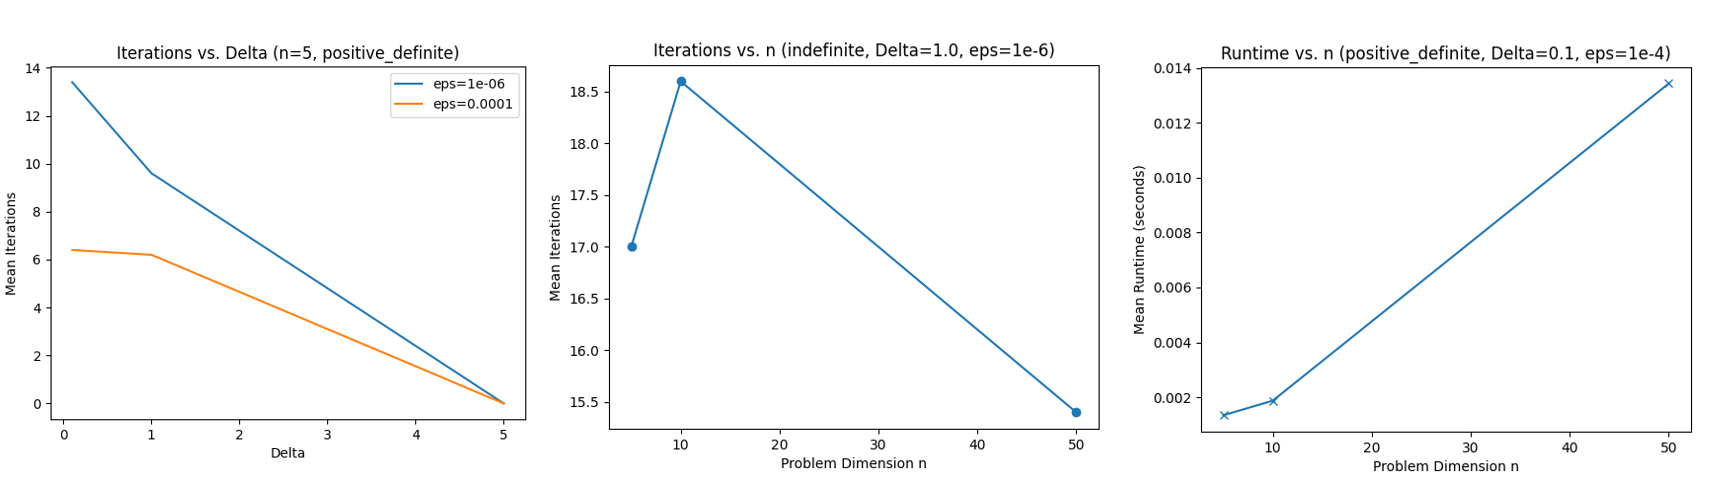
\includegraphics[width=1.25\textwidth]{pics/h6/6.png}}
    \caption{Benchmark}
    \label{fig:6}
\end{figure}
\FloatBarrier
For fixed $\Delta=1.0$ and indefinite $Q$, iteration count grows slowly with $n$, confirming the dimension-agnostic nature of bisection. Runtime increases with $n$ due to matrix factorization in each iteration. However, for $n=50$, the solve time remained acceptable (milliseconds). A stricter tolerance ($\epsilon=10^{-6}$) increased iteration count by 2--5 steps compared to $\epsilon=10^{-4}$. The difference was more pronounced when the solution lay near the boundary.

\subsection{Experimental Shortcomings}

\textbf{Near-Singular Cases:} If $Q+ \lambda I$ becomes nearly singular for small $\lambda$, we might see numerical instability. In practice, we observed a few LinAlgError expansions but no major breakdown.\\
\textbf{Random Data:} Our indefinite or negative definite matrices are artificially generated, which may differ from real-world data (where structures like sparsity or specific eigenvalue distributions matter). Future work might test structured or extremely large $n$.





\section{Conclusion}

%What knowledge have we gained?
%Could we answer the question we set out to answer in the Introduction?

Through extensive experiments and theoretical analysis, we have demonstrated that Algorithm 12 effectively solves the trust-region subproblem across a wide range of conditions. The algorithm reliably produces solutions that satisfy both the norm constraint and the KKT optimality conditions, with feasibility errors and residuals consistently near machine precision. The method exhibits robust and predictable performance, with iteration counts and runtimes scaling moderately with problem size. The bisection approach used for adjusting the Lagrange multiplier $\lambda$ achieves linear convergence and ensures numerical stability even when the problem is indefinite. Overall, Algorithm 12 is a reliable and efficient method for norm-constrained quadratic optimization in low to moderate dimensions.
\end{document}
